\begin{figure}[h]
    \centering
    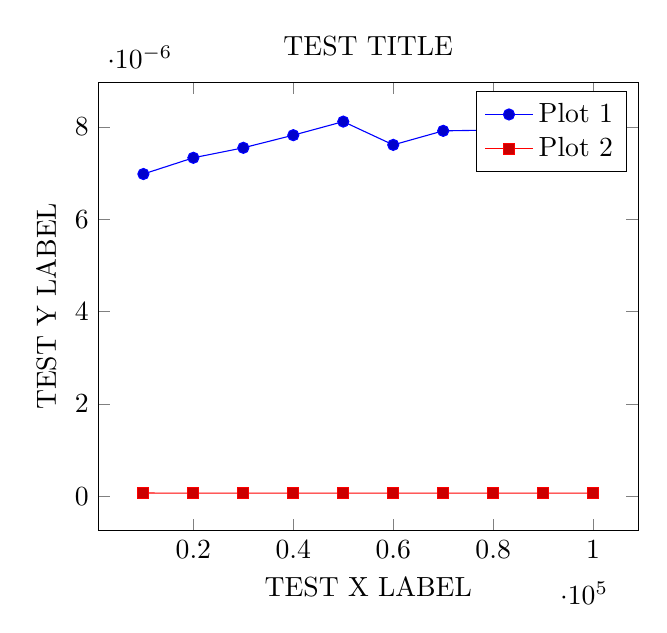
\begin{tikzpicture}
        \begin{axis}[
            xlabel={TEST X LABEL},
            ylabel={TEST Y LABEL},
            title={TEST TITLE}
        ]
		\addplot coordinates {
			(10000, 6.981244305903745e-06)
			(20000, 7.332715923892952e-06)
			(30000, 7.54865864034393e-06)
			(40000, 7.822125846114414e-06)
			(50000, 8.116072974783783e-06)
			(60000, 7.612206636398611e-06)
			(70000, 7.916092551180975e-06)
			(80000, 7.932657194702265e-06)
			(90000, 7.858266886524579e-06)
			(100000, 8.160646924623371e-06)
		};
		\addplot coordinates {
			(10000, 7.408913284123741e-08)
			(20000, 7.107737947364967e-08)
			(30000, 7.137855481031963e-08)
			(40000, 7.258325615699946e-08)
			(50000, 7.137855481031963e-08)
			(60000, 7.137855481031963e-08)
			(70000, 7.22820808203295e-08)
			(80000, 7.167973014654549e-08)
			(90000, 7.198090548365955e-08)
			(100000, 7.22820808203295e-08)
		};
        \legend{Plot 1, Plot 2}
        \end{axis}
    \end{tikzpicture}
    \caption{TEST CAPTION}
\end{figure}